\chapterimage{anhang.png}
\chapter{Anhang}
\label{chap:appendix}

\section{Anhang 1: Struktur der Befragung}
\label{anhang:fragebogen}
\paragraph{Opener}
\begin{itemize}
    \item Studenten am KIT
    \item Seminar
    \item Wollten Sie kurz fragen: \textbf{Wie schenken Sie?}
\end{itemize}

\paragraph{Fragenkatalog falls es nicht mehr weiter geht}
\begin{enumerate}
    \item Wann machen Sie sich zum ersten Mal Gedanken über die Weihnachtsgeschenke?
    \item Woher bekommen Sie ihre Ideen?
    \item Was beeinflusst Ihre Entscheidung für den Kauf?
    \item Wie kommen Sie an Ihre Geschenke?  Wann und Wo?
    \item Wie verpacken Sie Ihre Geschenke?  Wann?
    \item Wie läuft bei Ihnen die Bescherung ab?
\end{enumerate}

\paragraph{Wichtige Fragen vor dem Ende}
\begin{enumerate}
    \item Verhältnis zu Weihnachten (falls notwendig)
    \item Wichtigkeit des Schenkens
    \item Zufriedenheit mit Ihren Geschenken die Sie schenken
    \item Ihr Alter
    \item Ihre Kontaktdaten
\end{enumerate}

\paragraph{Antwort Maske}
\begin{figure}[!h]
    \centering
      \makebox[\textwidth]{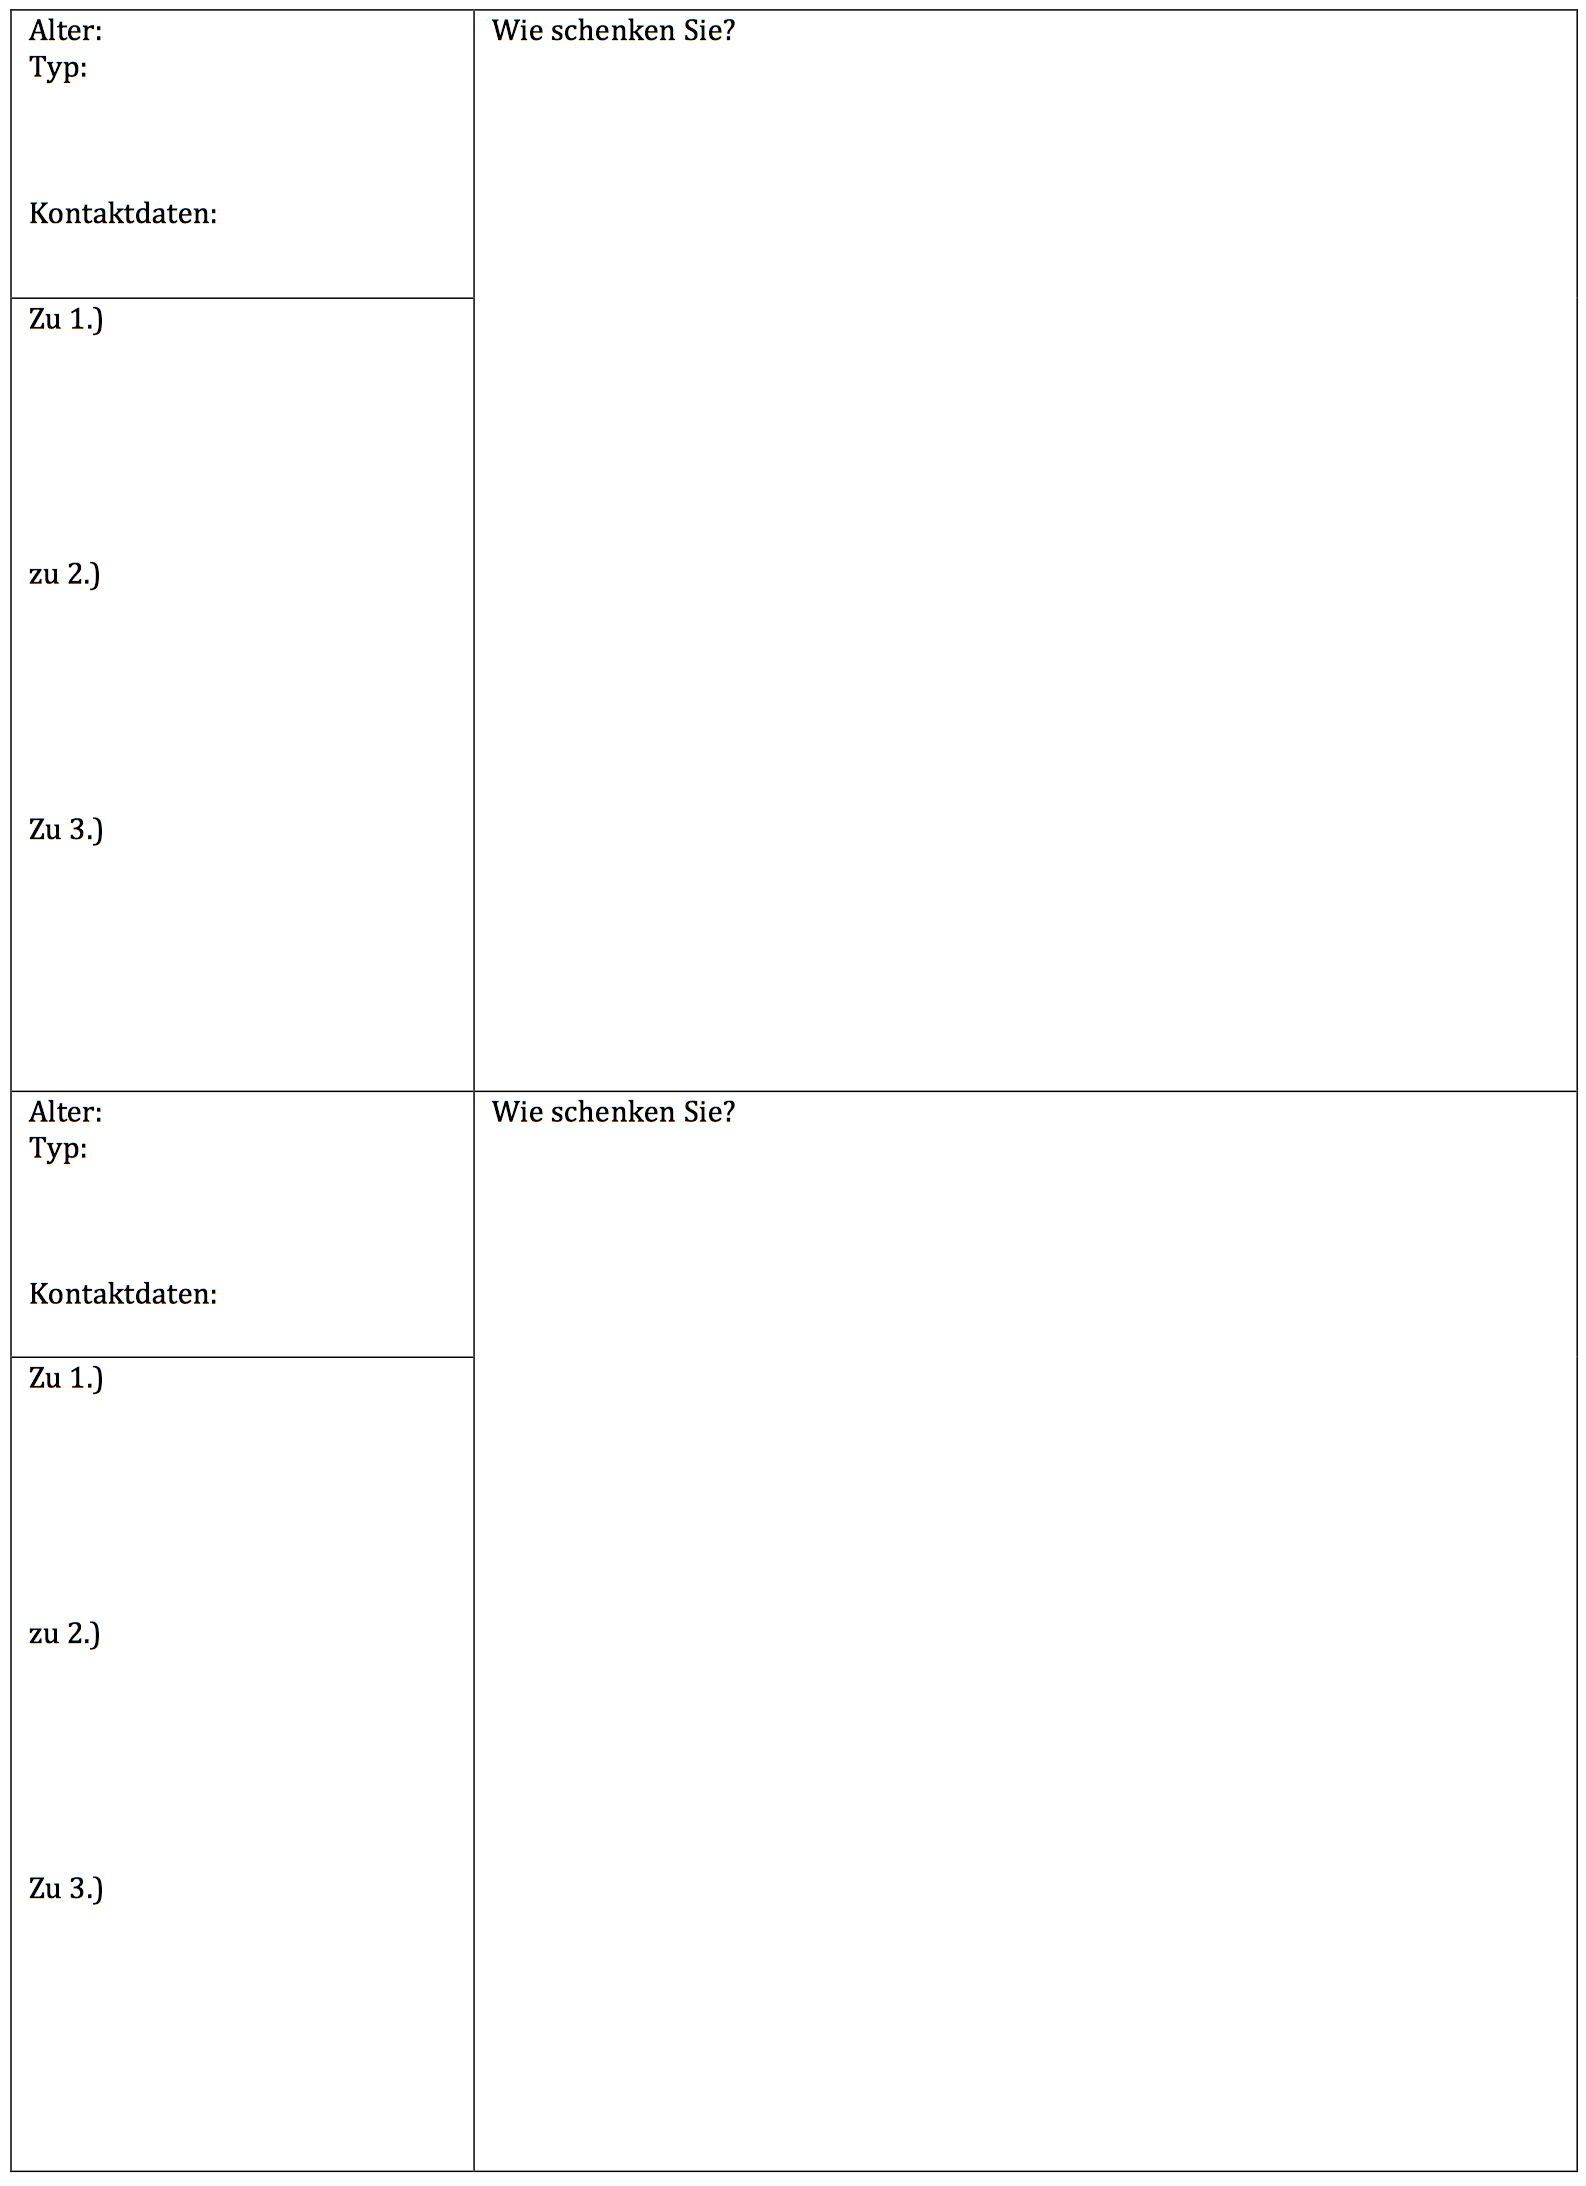
\includegraphics[width=0.8\textwidth]{fragen}}
    \caption{Antwort Maske}
    \label{fig:maske}
\end{figure}

\newpage

\section{Anhang 2: Personae}
\label{anhang:Personae}
\paragraph{Der Pragmatiker}

\textbf{Name & Alter:} Sven Müller, 39 Jahre\\
\textbf{Familien- und sozialer Status:} Verheiratet, Vater von 2 Söhnen\\
\textbf{Stadt:} München\\
\textbf{Beruf & Einkommen:} Arbeitet im Controlling eines mittelständigen Unternehmens, etwa \EUR{65.000}\\
\hline
\paragraph{Rolle & Position im Stakeholder-Netzwerk:}
Sven Müller ist Alleinverdiener im Haushalt, da seine Frau sich z.Zt. in Elternurlaub befindet. Er selbst sieht sich als „Brötchenverdiener“ der Familie und sieht sich deshalb auch in der Position des Familienoberhaupts. Im Beruf befindet er sich im mittleren Management. Da er aufsteigen möchte engagiert er sich intensiv im Beruf. Er engagiert sich zudem in seinem Musikverein und ist dort, vorteilhaft durch seinen Beruf, Finanzer.\\
\hline
\paragraph{Hobbies & Identifizierungsmaßnahmen:}
Sven Müller fährt sehr gerne im Sommer mit seinem Motorrad. Aufgrund der Nähe zu den Alpen unternimmt er im Sommer an verlängerten Wochenenden öfters dort eine Tour, welche über das ganze Wochenende dauert. Als Stressausgleich und aufgrund der mangelnden Bewegung in seinem Job führt er seinen Hund abends nach der Arbeit für eine größere Runde Gassi. In der Musikkapelle seines Vorortes spielt er erstes Saxophon. Das bedeutet für ihn zum einen regelmäßiges Üben, und zum anderen die Teilnahme an Konzerten. Gleichzeitig jedoch auch ein Zeitaufwand.\\
\hline
\paragraph{Pain Points & Needs / Einstellung gegenüber ... (brand, service, problem, topic):}
Sven Müller fühlt sich als ob er an mehreren Baustellen gleichzeitig arbeiten müsste. Trotz des Elternurlaubs der Frau möchte er gleichzeitig den gleichen Standard für die Familie halten. Hinzu kommt, dass die Arbeit ihm auch für die persönliche Weiterentwicklung wichtig ist, da er Karriere machen möchte. Diesen Stress möchte er durch sein Engagement im Musikverein und durch seine Hobbys lösen, was ihm durchaus gelingt. Die Familie ist für ihn zentraler Haltepunkt seines Lebens, weshalb ihm die Zeit mit seiner Frau und den Söhnen wichtig ist. Durch die Arbeit und sein Engagement kommt das inzwischen zu kurz, weshalb eines seiner zentralen Bedürfnisse ist, mehr Zeit für die Familie zu haben.\\
Weihnachten steht er positiv gegenüber. Für ihn ist es eine Zeit des Jahres, in der er sich voll und ganz seiner Familien widmen kann. Da er jedoch sehr beschäftigt ist, möchte er bei der Organisation des Festes nicht mitwirken. Ihm sind nur ein paar wenige Rahmenbedingungen wichtig, auf die er sich vorher mit seiner Frau geeinigt hat. Das Schenken ist ein weiterer, für ihn zeitraubender, Schritt, den er nur ungern jedes Jahr aufs Neue macht, ihm jedoch sehr wichtig ist. Er schenkt nur seiner Familie und dem engsten Freundeskreis etwas, steht aber jedes Jahr vor dem Problem, dass er keine Zeit hat einzukaufen oder sich etwas zu überlegen. Aus diesem Grund fragt er entweder verdeckt oder offen nach, was die Beschenkten möchten. Er hat das Gefühl, dass dieses Verhalten den Beschenkten nicht direkt gefällt, weshalb er nach Auswegen sucht, dies anders zu machen ohne dabei viel mehr Aufwand zu investieren.\\
\hline
\paragraph{Ziele & Träume:}
Sven Müllers Ziel ist es, dass er wieder mehr Zeit für die Familie hat. Er möchte die Karrierestufe aufsteigen, hat jedoch nicht das Bedürfnis, ganz oben anzukommen. Sobald er ein ausreichendes Niveau erreicht hat, genügt ihm das. Er will an seinem Engagement im Musikverein festhalten, da ihm dies sozialen Ausgleich zu Arbeitskollegen und Familie gibt. Insgesamt wünscht er sich ein ausgeglicheneres, stressfreieres Leben.\\
\hline
\vspace*{0.1in}
\textbf{Drei Dinge, ohne die er nicht Leben kann:} Seine Familie, sein Hund und sein Saxophon \\
\textbf{Ich bin gut in:} Controlling, Saxophon\\
\textbf{Ich wünschte ich wäre gut in:} Golf \\
\textbf{Mein nächstes großes Event wird:} Mein 40. Geburtstag \\
\textbf{Mein Traumurlaub war:} Zwei Wochen in einer Ferienhütte in einem Fjord in Norwegen \\
\textbf{In meinem Kühlschrank ist immer:} Bier \\
\hline

\paragraph{Der Grinch}
\textbf{Name & Alter:} Christian Feldmann, 43 Jahre\\
\textbf{Familien- und sozialer Status:} Geschieden, einen Sohn\\
\textbf{Stadt:} Stuttgart\\
\textbf{Beruf & Einkommen:} LKW Fahrer, etwa \EUR{35.000}\\
\hline
\paragraph{Rolle & Position im Stakeholder-Netzwerk:}
Christian Feldmann ist geschieden und sein Sohn, 21 Jahre, wuchs bei seiner Mutter auf. Die Beziehung zu ihm beschreibt er als abgekühlt, jedoch sehen sie sich regelmäßig. In seinem Beruf hat er nur wenig Kontakt zu seinen Kollegen. Er spielt keine zentrale Rolle im Unternehmen, ist jedoch stolz auf seinen Beruf und seine Arbeit. Als alteingesessener Fan des VfB Stuttgart trifft er sich zu den zweiwöchentlichen Heimspielen mit Gleichgesinnten im Stadion und an den anderen Wochenende zum Fußballschauen in seiner Stammkneipe (AnnehmBAR). Diese besucht er öfters, da dort seine Freundeskreis ist, mit denen er Karten spielt.\\
\hline
\paragraph{Hobbies & Identifizierungsmaßnahmen:}
Christian Feldmann ist Fan des VfB, den er als seine Liebe bezeichnen würde. Ihm ist wichtig, dass andere dies erkennen, weshalb er auch außerhalb von Spielen gelegentlich das Trikot oder den Schal trägt. Obwohl er seinen Job sehr gerne macht, ist er für ihn keine Identifizierung. Er könnte auch jeden anderen Job machen, wenn er dafür qualifiziert ist. Wichtig ist ihm das Kartenspielen, da es ihn mit seinen engsten Freunde zusammenbringt.\\
\hline
\paragraph{Pain Points & Needs / Einstellung gegenüber ... (brand, service, problem, topic):}
Christian Feldmanns mäßiges Verhältnis zu seinem Sohn bedrückt ihn sehr. Obwohl sie sich regelmäßig sehen, hat sich der Sohn in eine andere Richtung entwickelt und scheint, nach Christans Ansicht, sich sehr von ihm zu unterscheiden. Früher waren beide öfters zusammen im Stadion, doch selbst die Liebe zum VfB hat der Sohn nicht übernommen. Zu seiner Exfrau hat er nur noch ein oberflächliches Verhältnis, das sich nur auf die Gespräche über den Sohn begrenzt. Sie hat inzwischen erneuet geheiratet und ist in die Vorstadt gezogen. Aufgrund seiner gescheiterten Ehe und dem schlechten Verhältnis zum Sohn fragt sich Christian des Öfteren, warum es so gekommen ist. Er sieht sich selbst als hart arbeitenden Menschen, der sich immer um die Familie gekümmert hat. Sein größtes Bedürfnis ist es, das zerrüttete Verhältnis zu seinem Sohn wieder aufzubauen.\\
Gegenüber Weihnachten hat er eine schlechte Einstellung. Seitdem er es nicht mehr mit der Familie feiert, feiert er gar kein Weihnachten mehr. Er weiß auch nicht mehr, was er den Menschen, die er langsam nicht mehr zu kennen glaubt, schenken soll, weshalb er es komplett lässt. Für ihn ist Weihnachten deshalb nur noch eine Zeit des Jahres, mit der er nichts anzufangen weiß. Da er die Kirche ablehnt, hinterfragt er auch die Tatsache, dass dieser Tag als christlicher Feiertag ein nationaler Feiertag ist. Zudem sieht er das Verhalten aller Menschen als scheinheilig an. An Weihnachten predigen sie die humanistischen Werte des Christentums, welche sie zu allen anderen Zeiten des Jahres nicht interessieren.\\
\hline
\paragraph{Ziele & Träume:}
Christian Feldmanns Ziele sind zum einen das bessere Verhältnis zu seinem Sohn. Gleichzeitig wäre er gerne wieder in einer festen Beziehung, da er an seiner Exfrau erkennt, dass dies ein Glücksfaktor im Leben sein kann. Sein Traum ist natürlich der Aufstieg des VfB in die erste Liga\\
\hline
\vspace*{0.1in}
\textbf{Drei Dinge, ohne die er nicht Leben kann:} Sein Sohn, VfB und die AnnehmBAR\\
\textbf{Ich bin gut in:} Benokkel (schwäbisches Kartenspiel) \\
\textbf{Ich wünschte ich wäre gut in:} Ein Vater sein, Fußballspielen \\
\textbf{Mein nächstes großes Event wird:}  \\
\textbf{Mein Traumurlaub war:} Die Fahrt mit Frau und Kind in einem VW Bus durch Südeuropa \\
\textbf{In meinem Kühlschrank ist immer:} Bier \\
\hline

\newpage

\section{Anhang 3: Ideen}
\label{anhang:ideen}

\begin{figure}[h!]
    \centering
      \makebox[\textwidth]{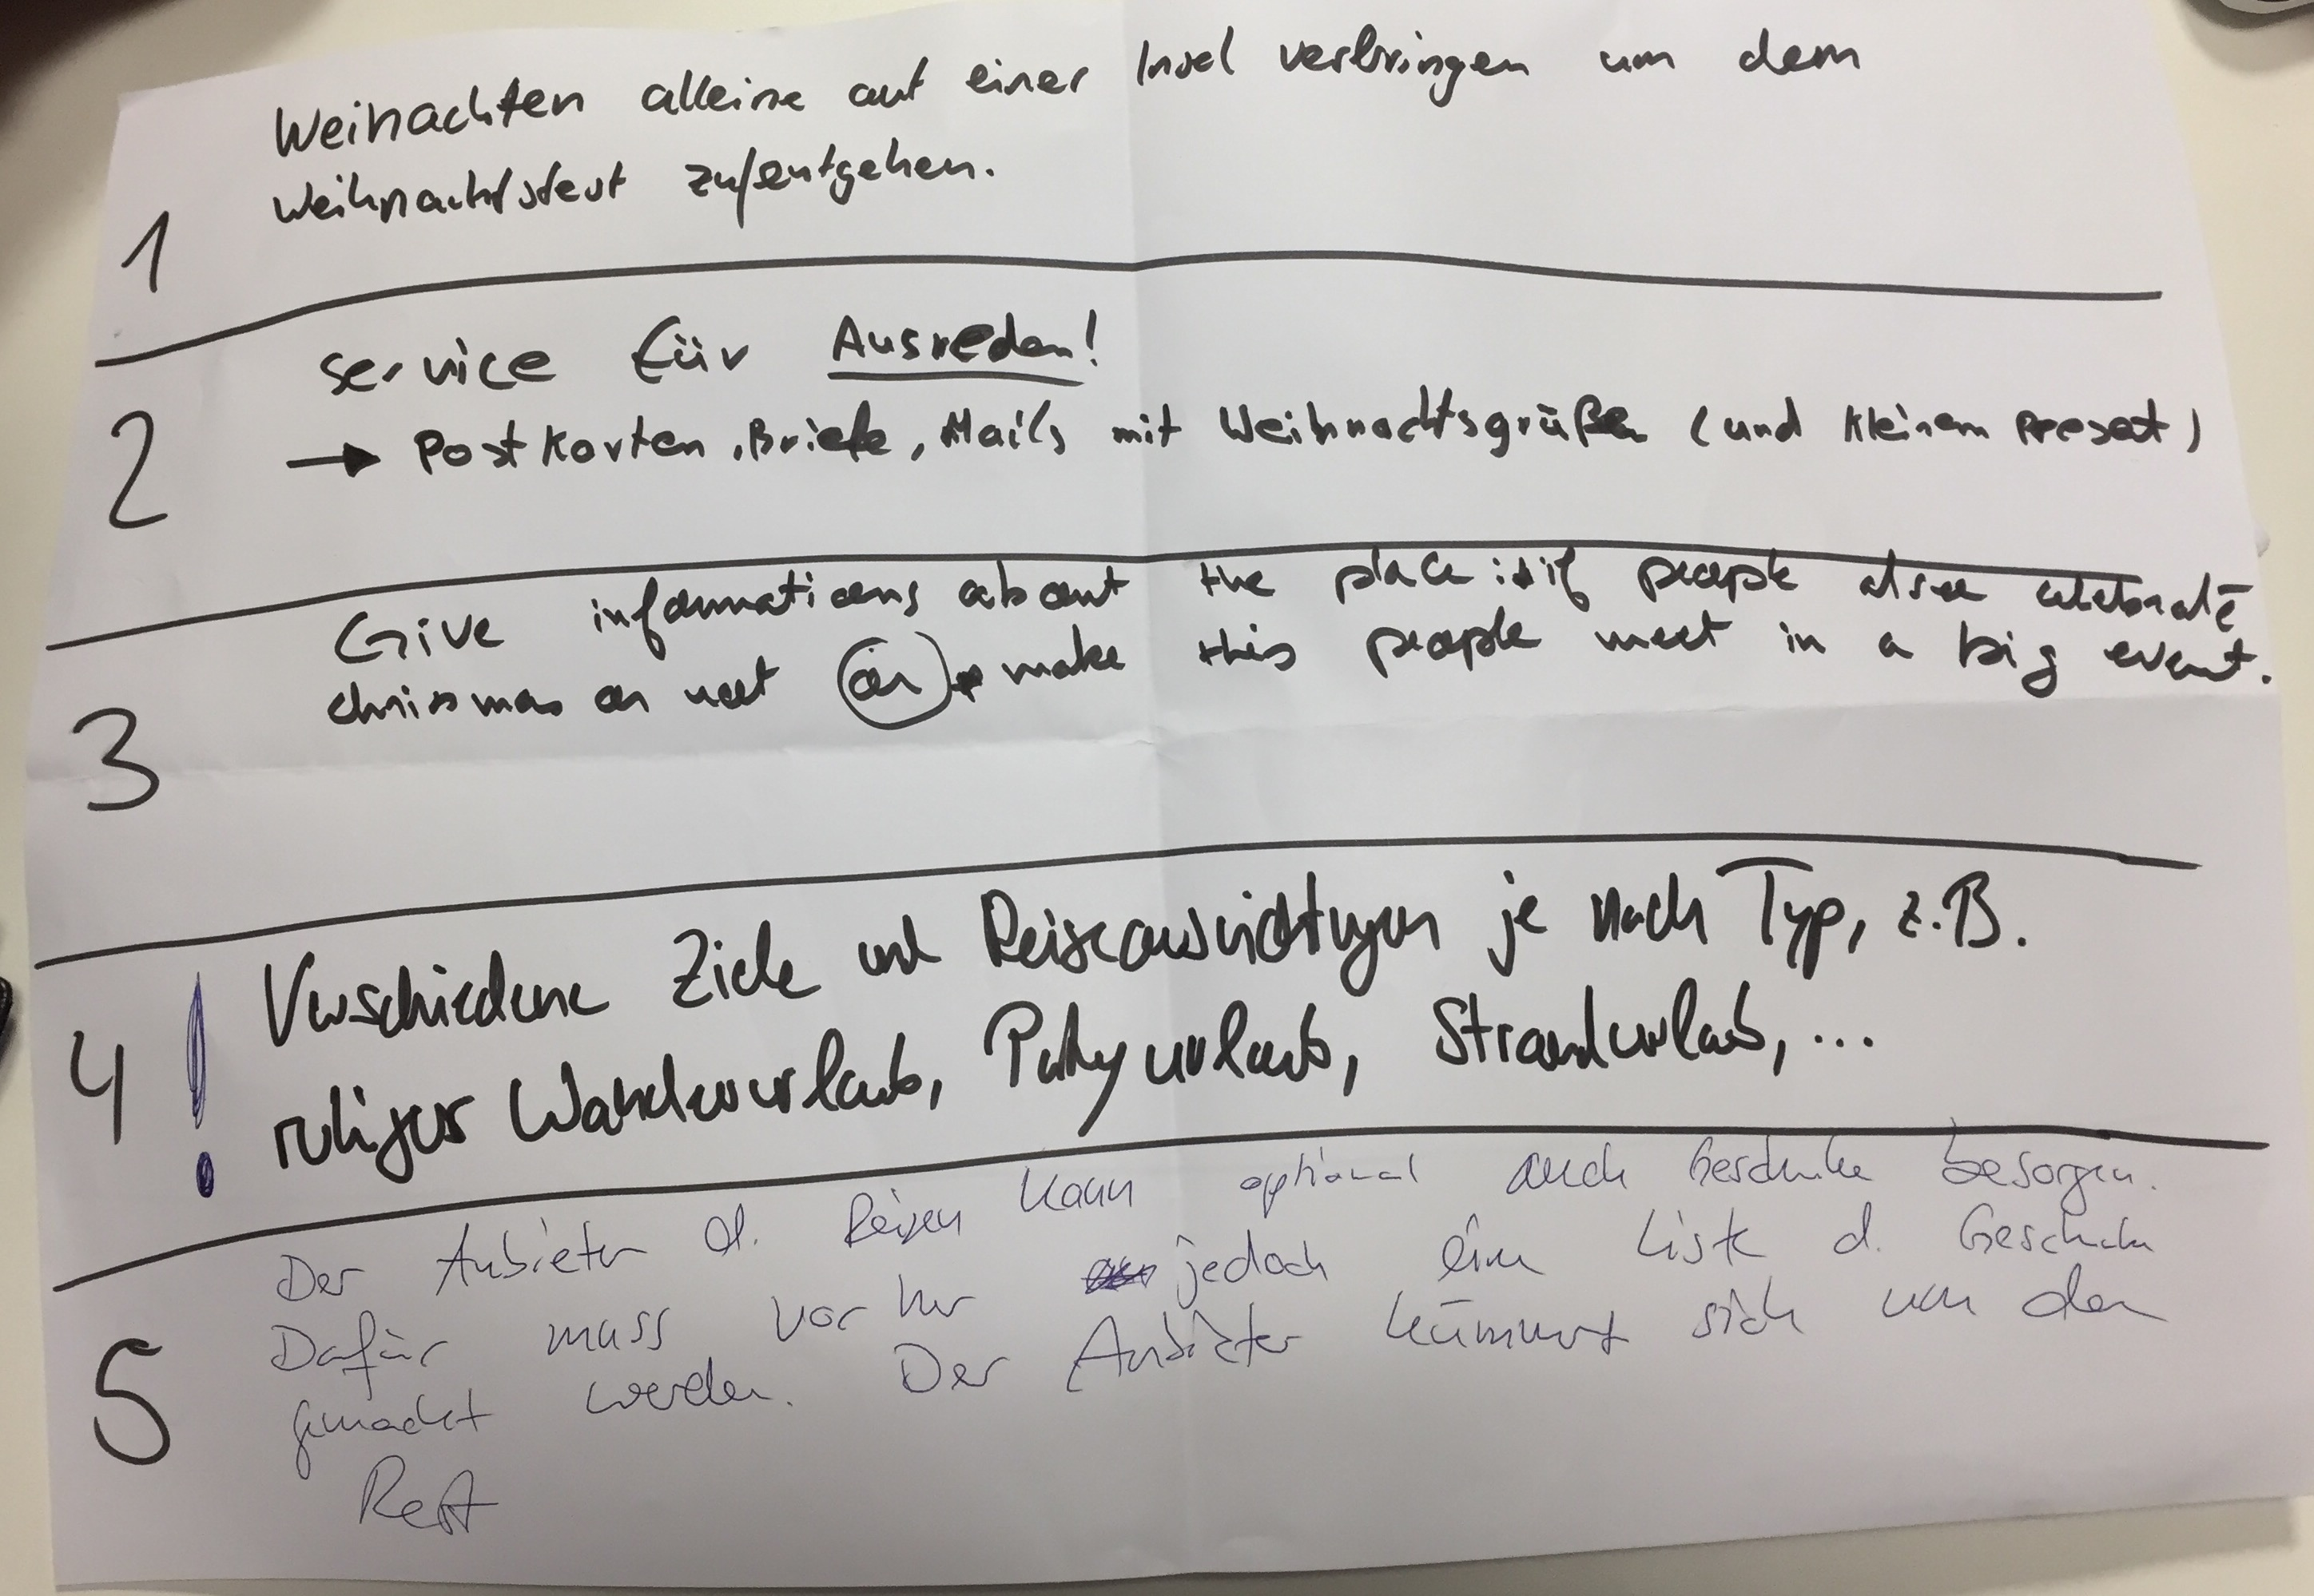
\includegraphics[height=0.3\paperheight]{idea1}}
    \caption{Idee 1}
    \label{fig:idea1}
\end{figure}

\begin{figure}[h!]
    \centering
      \makebox[\textwidth]{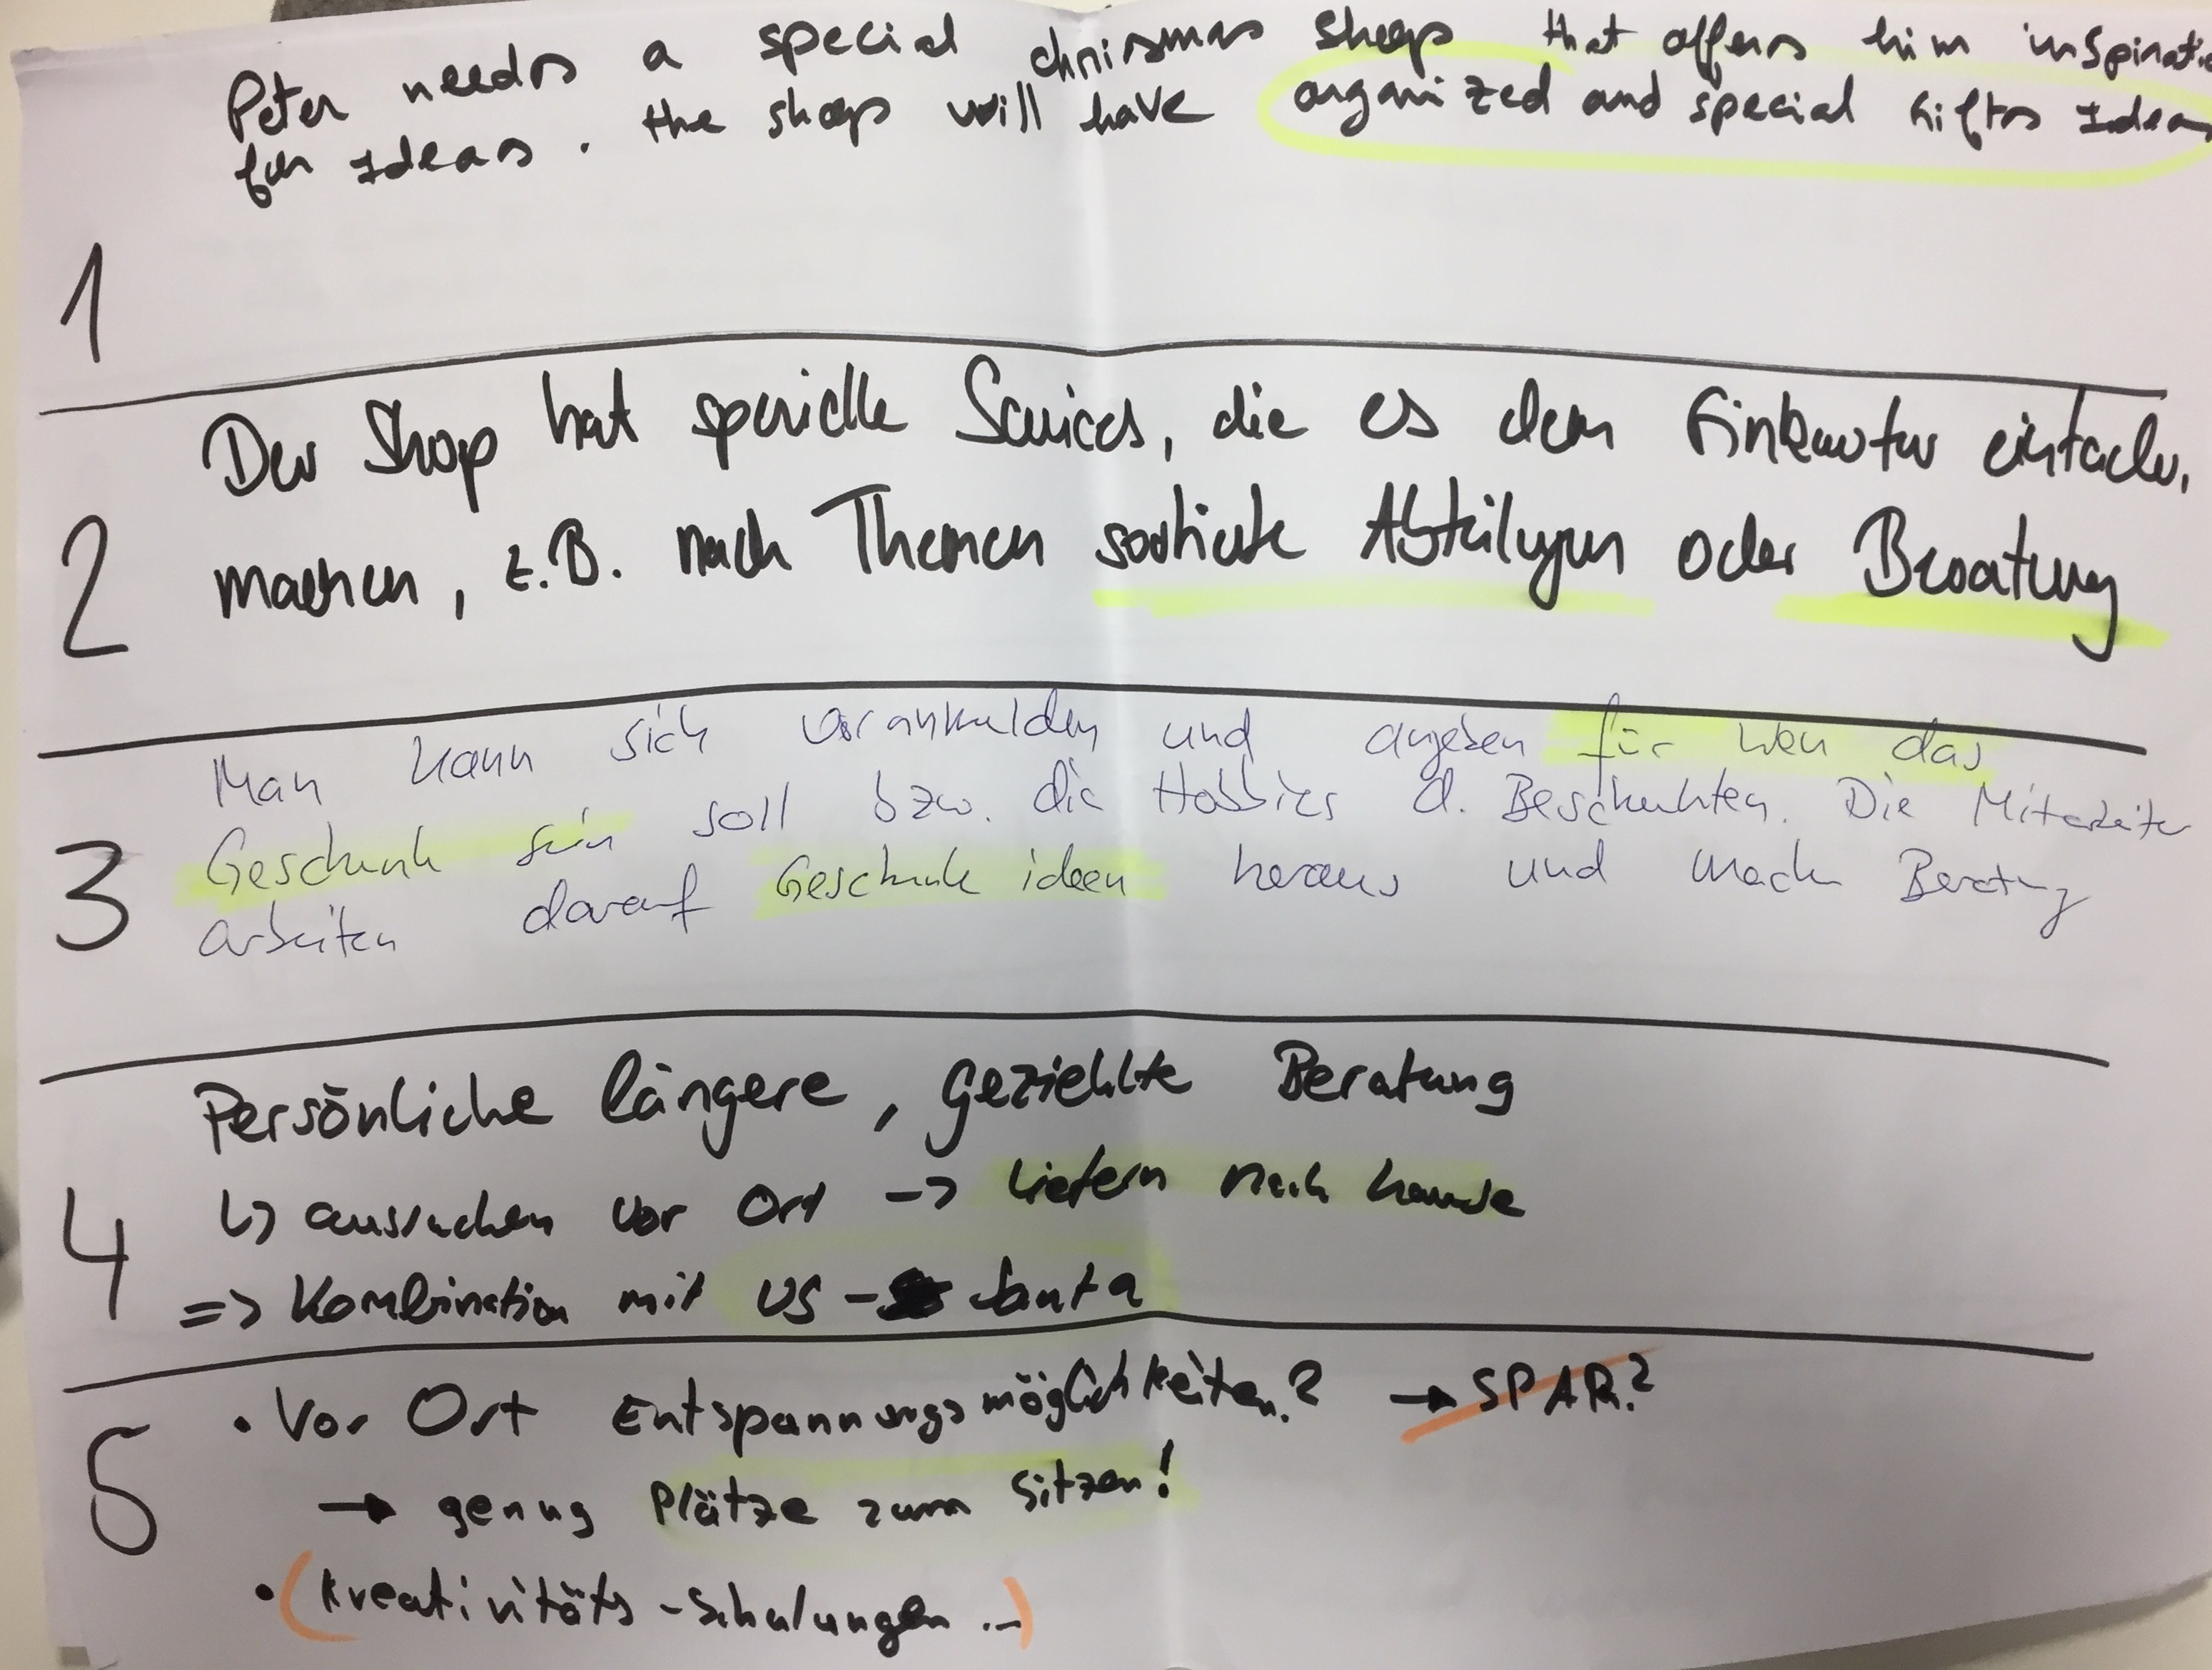
\includegraphics[height=0.3\paperheight]{idea2}}
    \caption{Idee 2}
    \label{fig:idea2}
\end{figure}

\begin{figure}[h!]
    \centering
      \makebox[\textwidth]{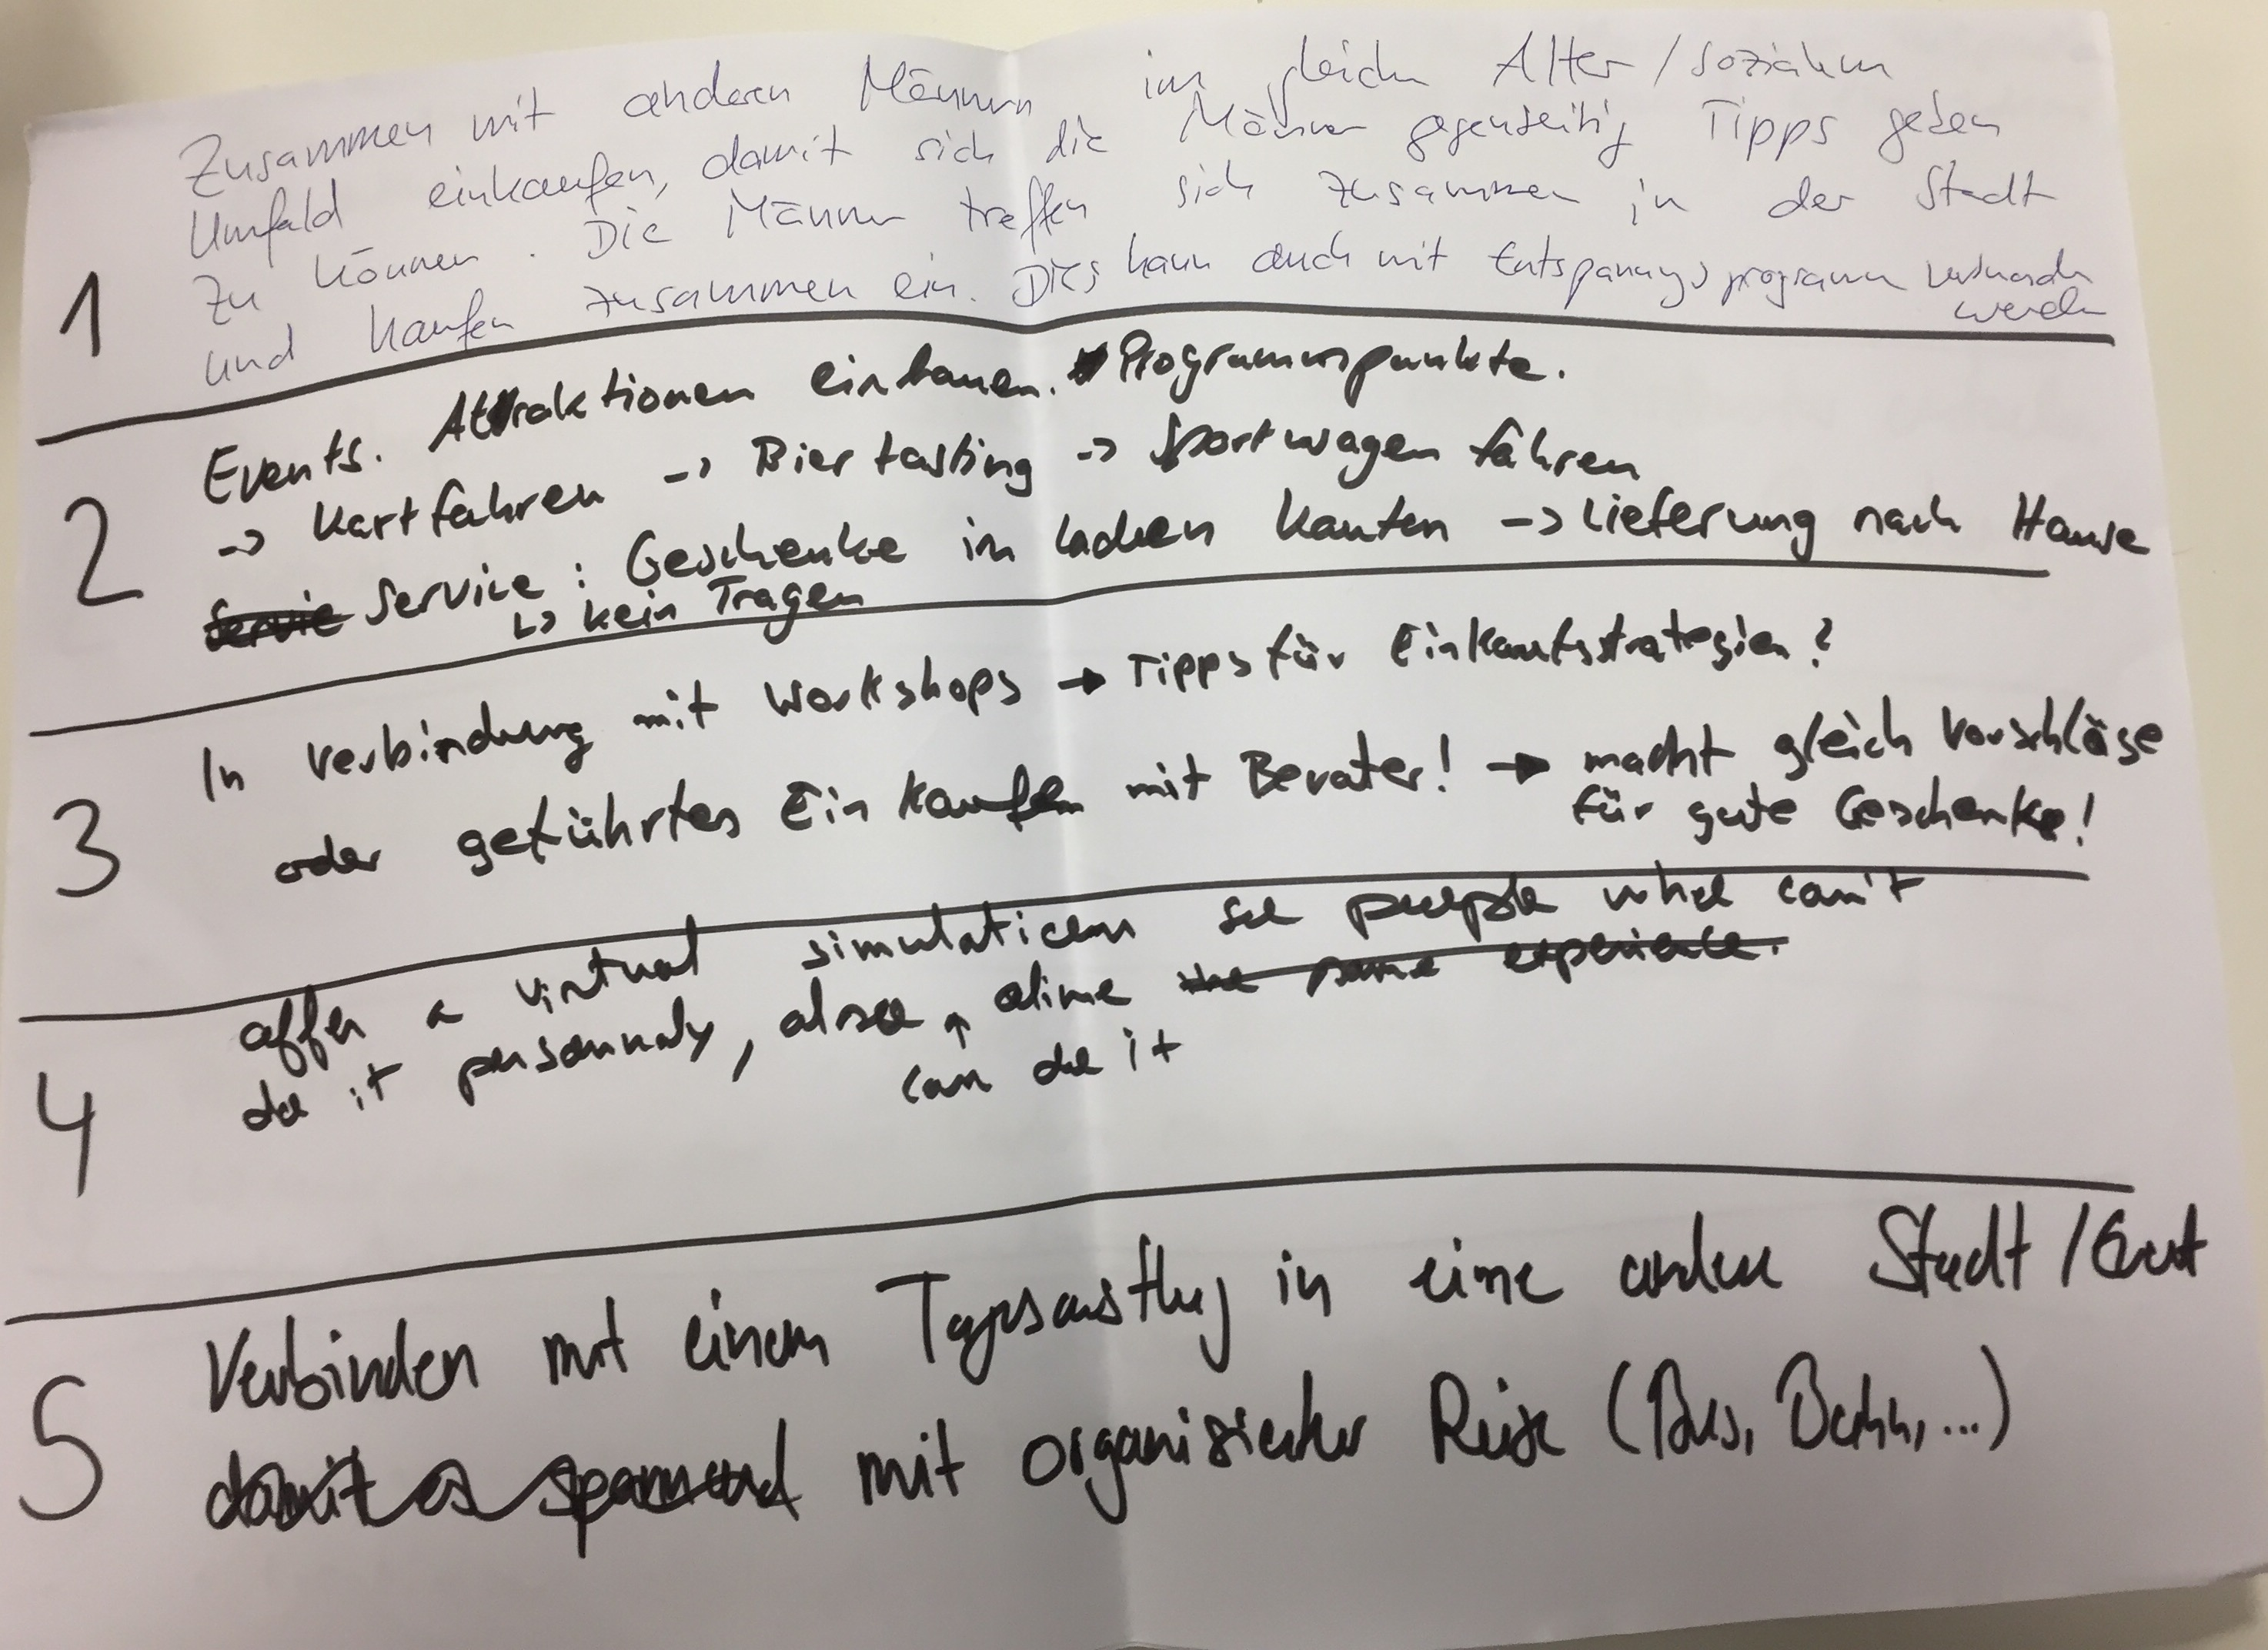
\includegraphics[height=0.3\paperheight]{idea3}}
    \caption{Idee 3}
    \label{fig:idea3}
\end{figure}

\begin{figure}[h!]
    \centering
      \makebox[\textwidth]{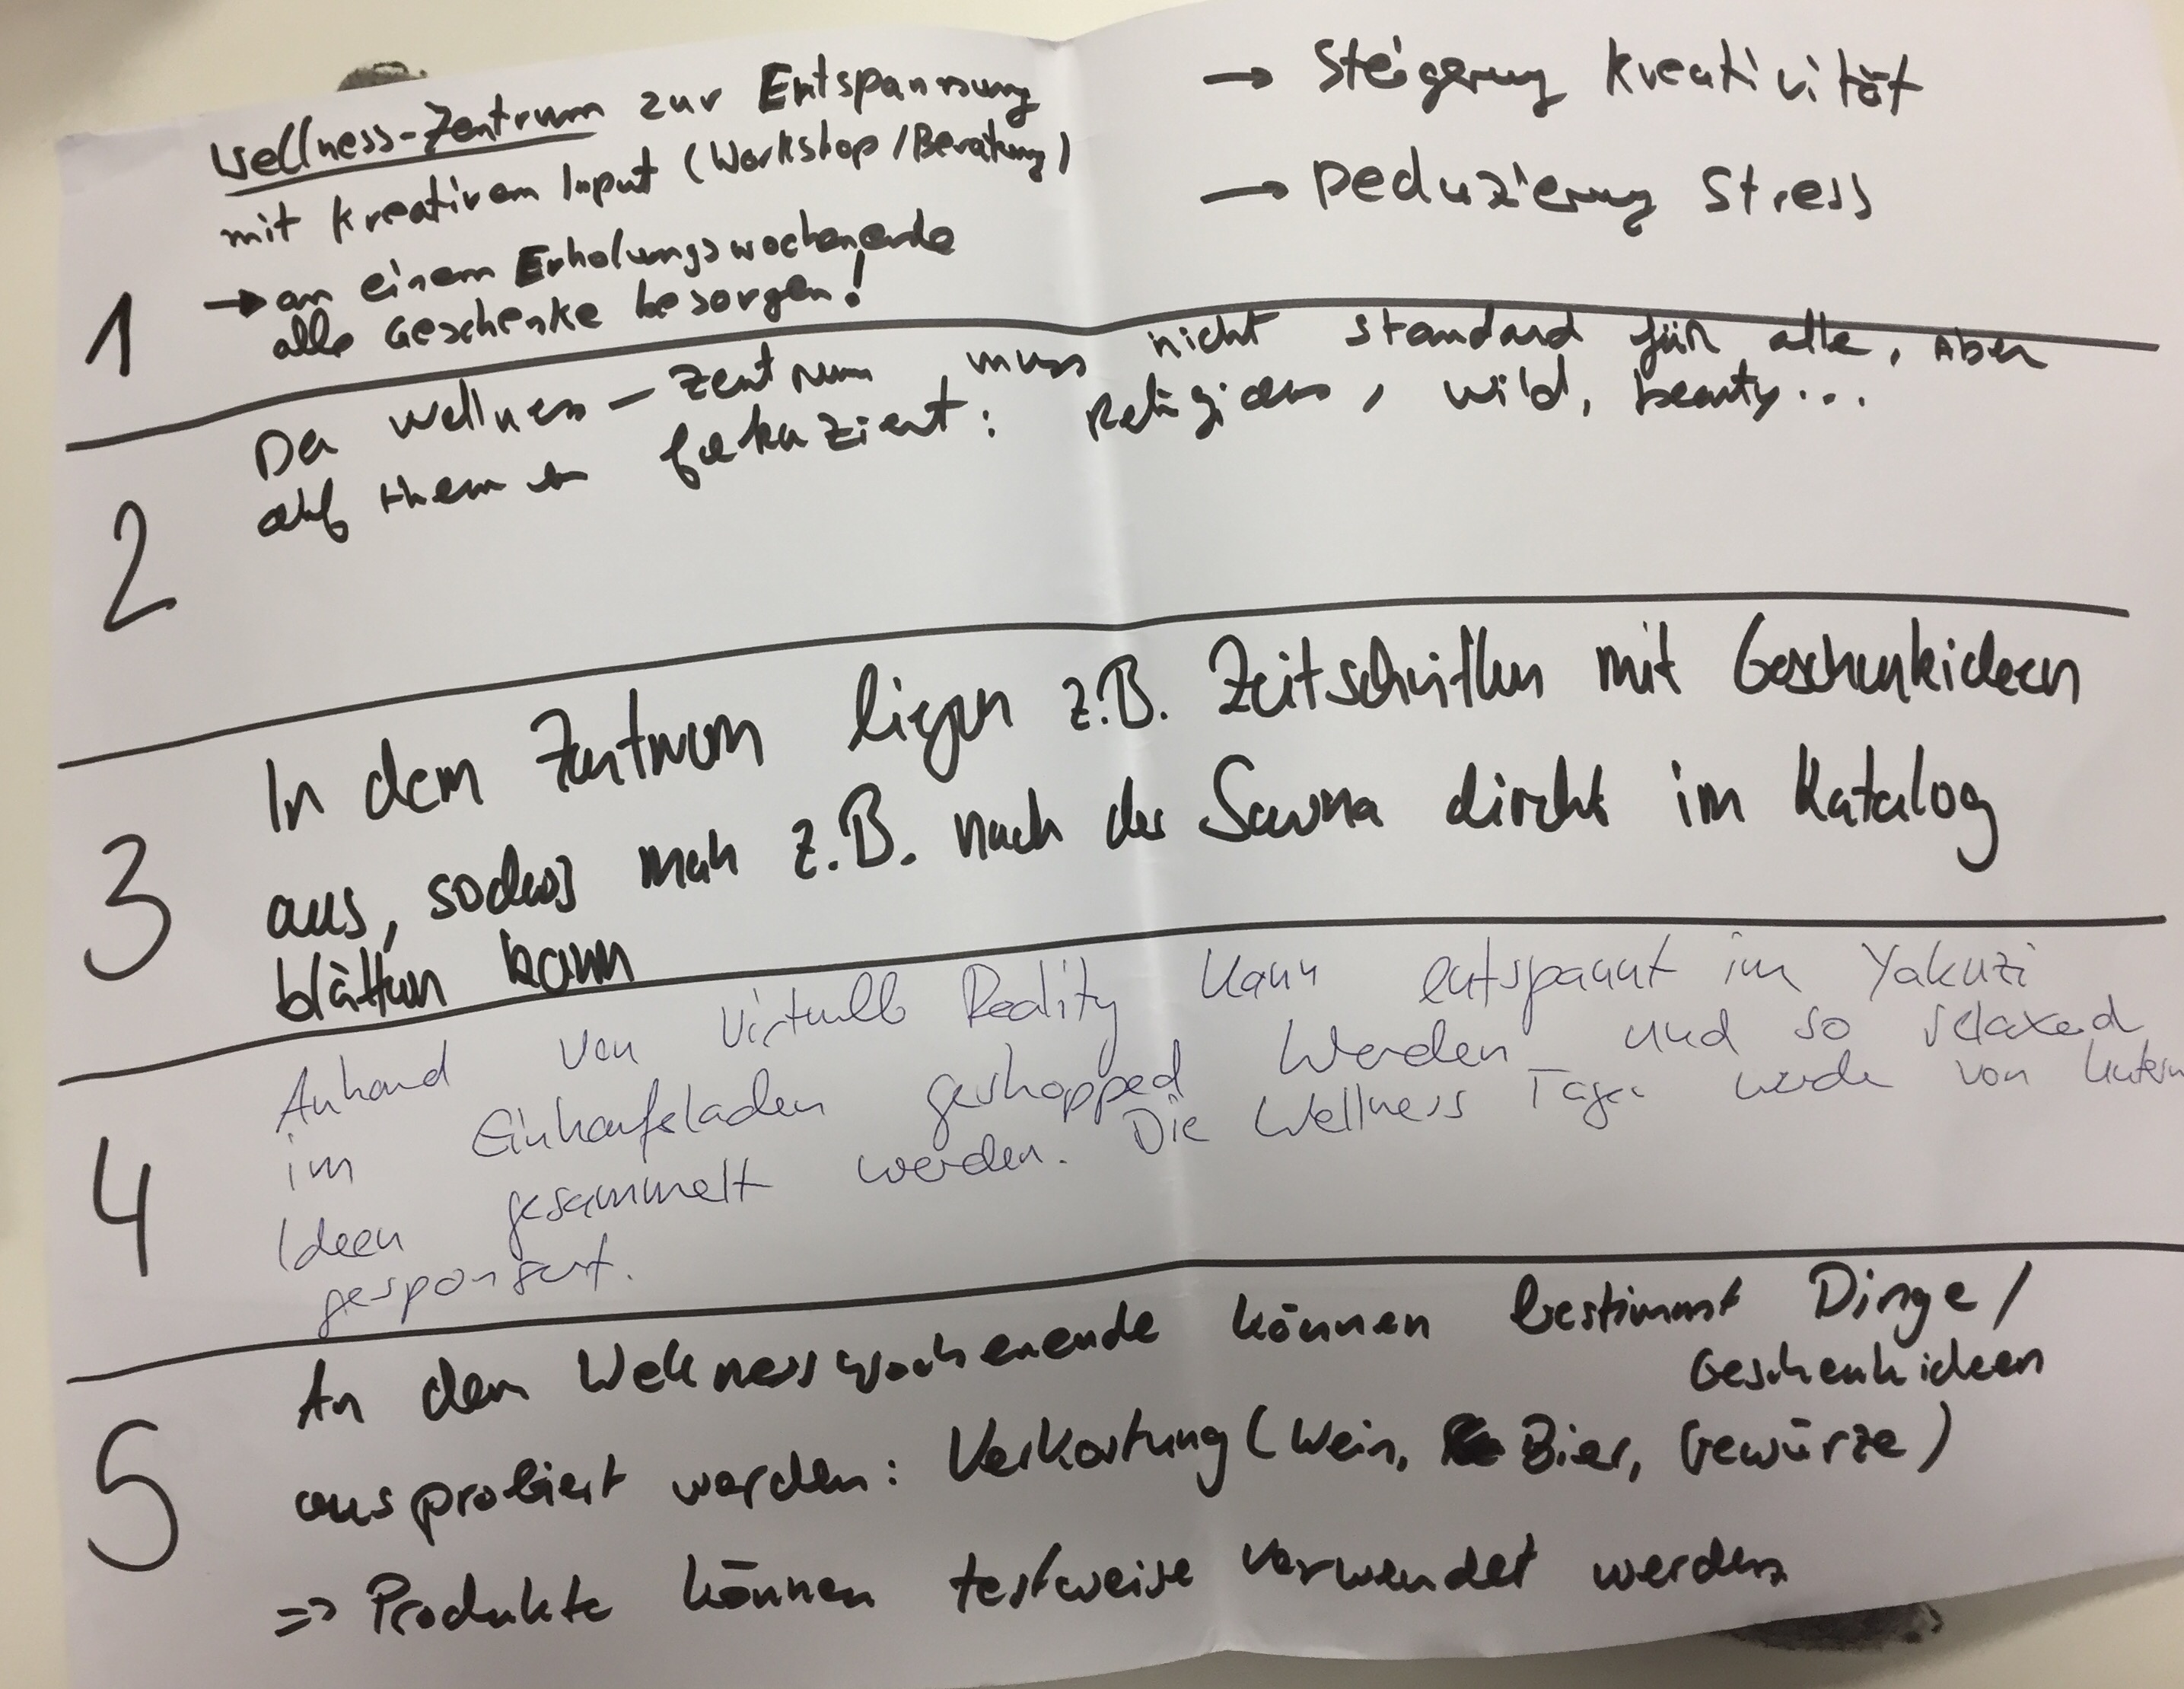
\includegraphics[height=0.3\paperheight]{idea5}}
    \caption{Idee 4}
    \label{fig:idea4}
\end{figure}


\begin{figure}[h!]
    \centering
      \makebox[\textwidth]{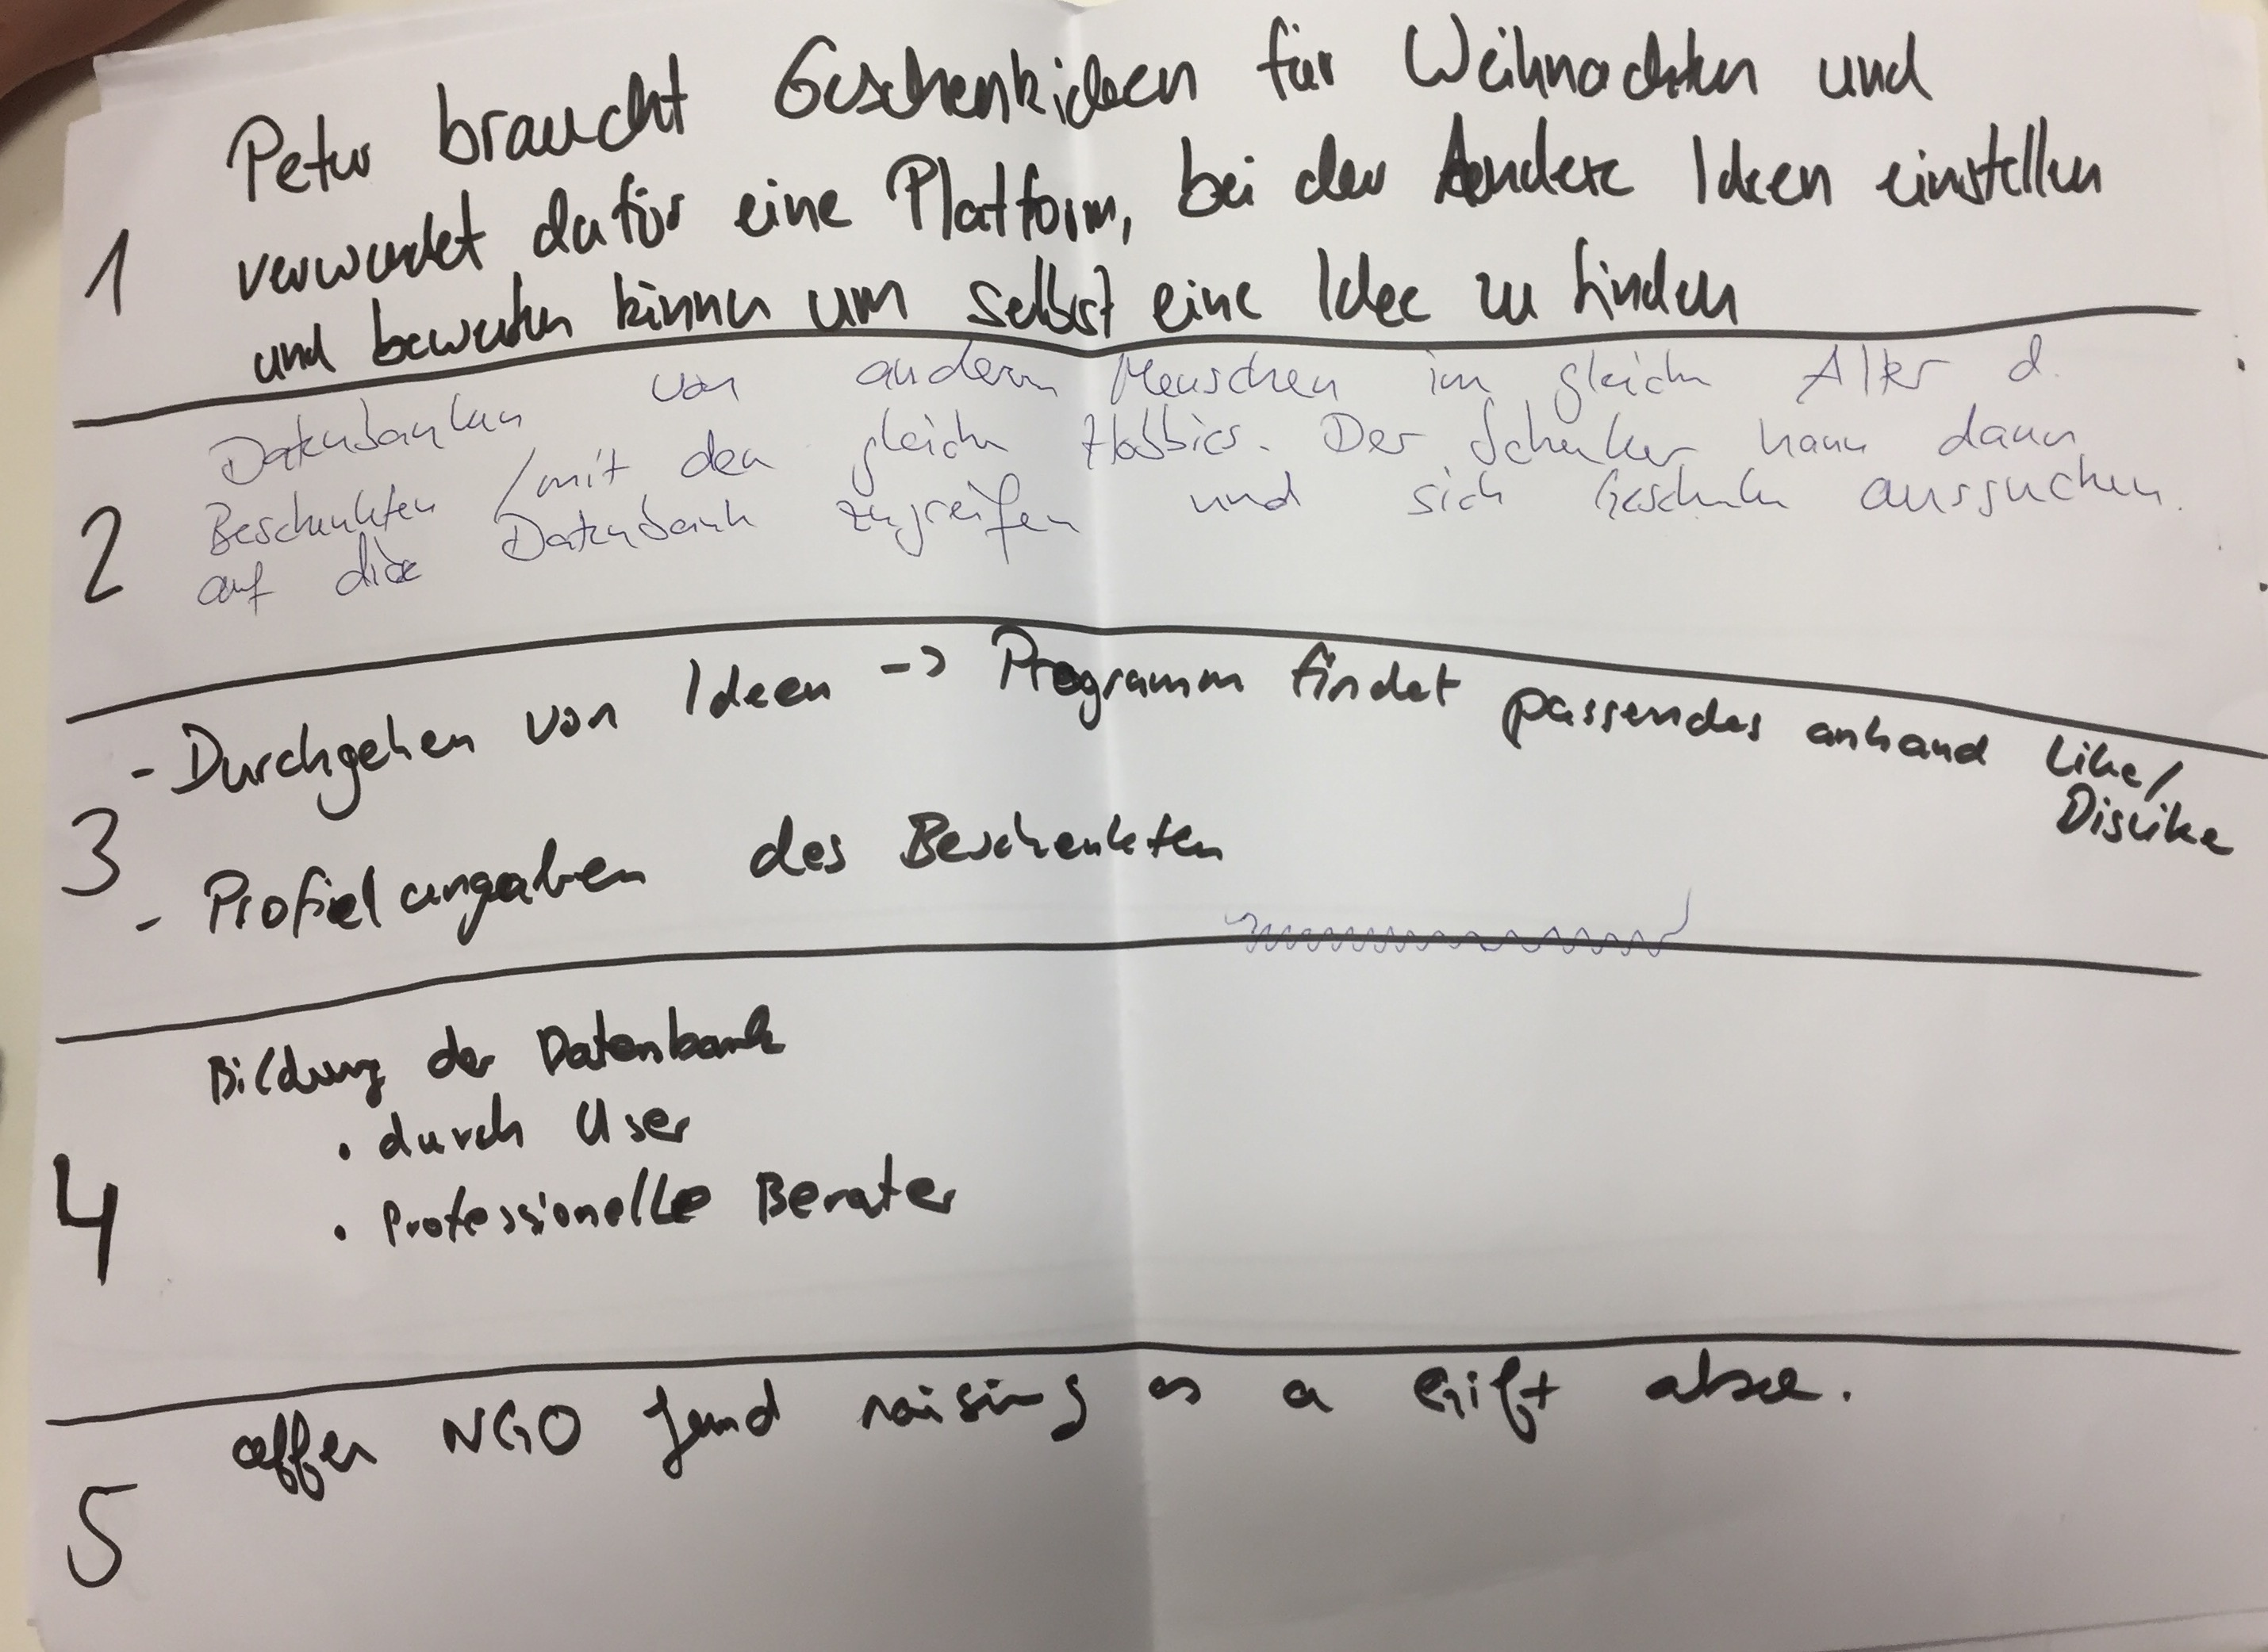
\includegraphics[height=0.35\paperheight]{idea4}}
    \caption{Idee 5}
    \label{fig:idea5}
\end{figure}

\vspace*{1in}

\newpage

\section{Anhang 4: Prototypen}
\label{anhang:protos}
Dieses Anhang enthält alle prototypen im größere Forme, damit der Leser detailierte blick auf alle Features haben kann.

\begin{figure}[ht]
    \centering
      \makebox[\textwidth]{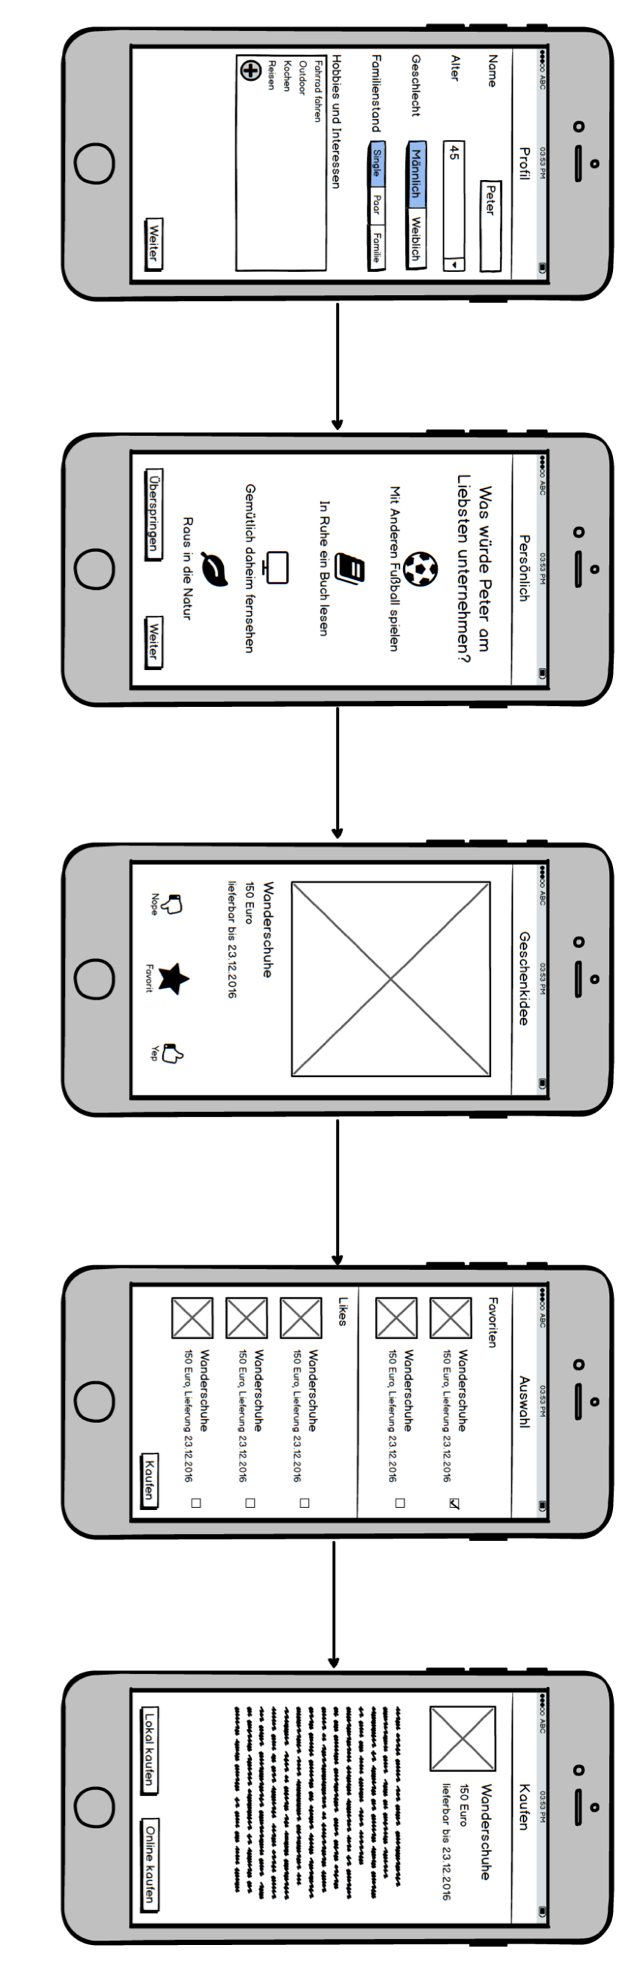
\includegraphics[height=0.83\paperheight]{prt1}}
    \caption{Swipe-App (Prototyp 1)}
    \label{fig:prt1}
\end{figure}

\begin{figure}[ht]
    \centering
      \makebox[\textwidth]{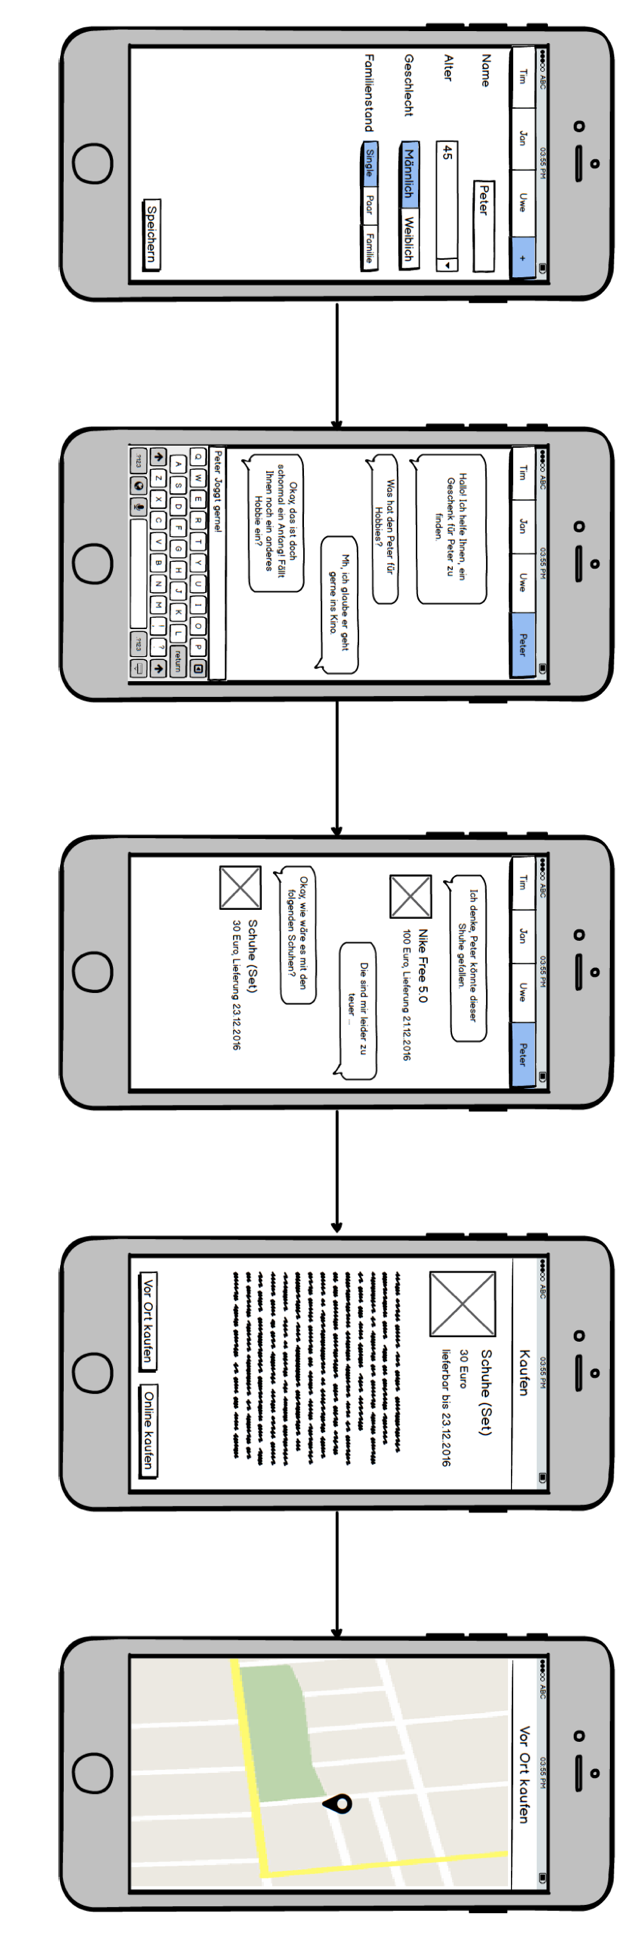
\includegraphics[height=0.83\paperheight]{prt2}}
    \caption{Chat-Bot (Prototyp 2)}
    \label{fig:prt2}
\end{figure}

\begin{figure}[ht]
    \centering
      \makebox[\textwidth]{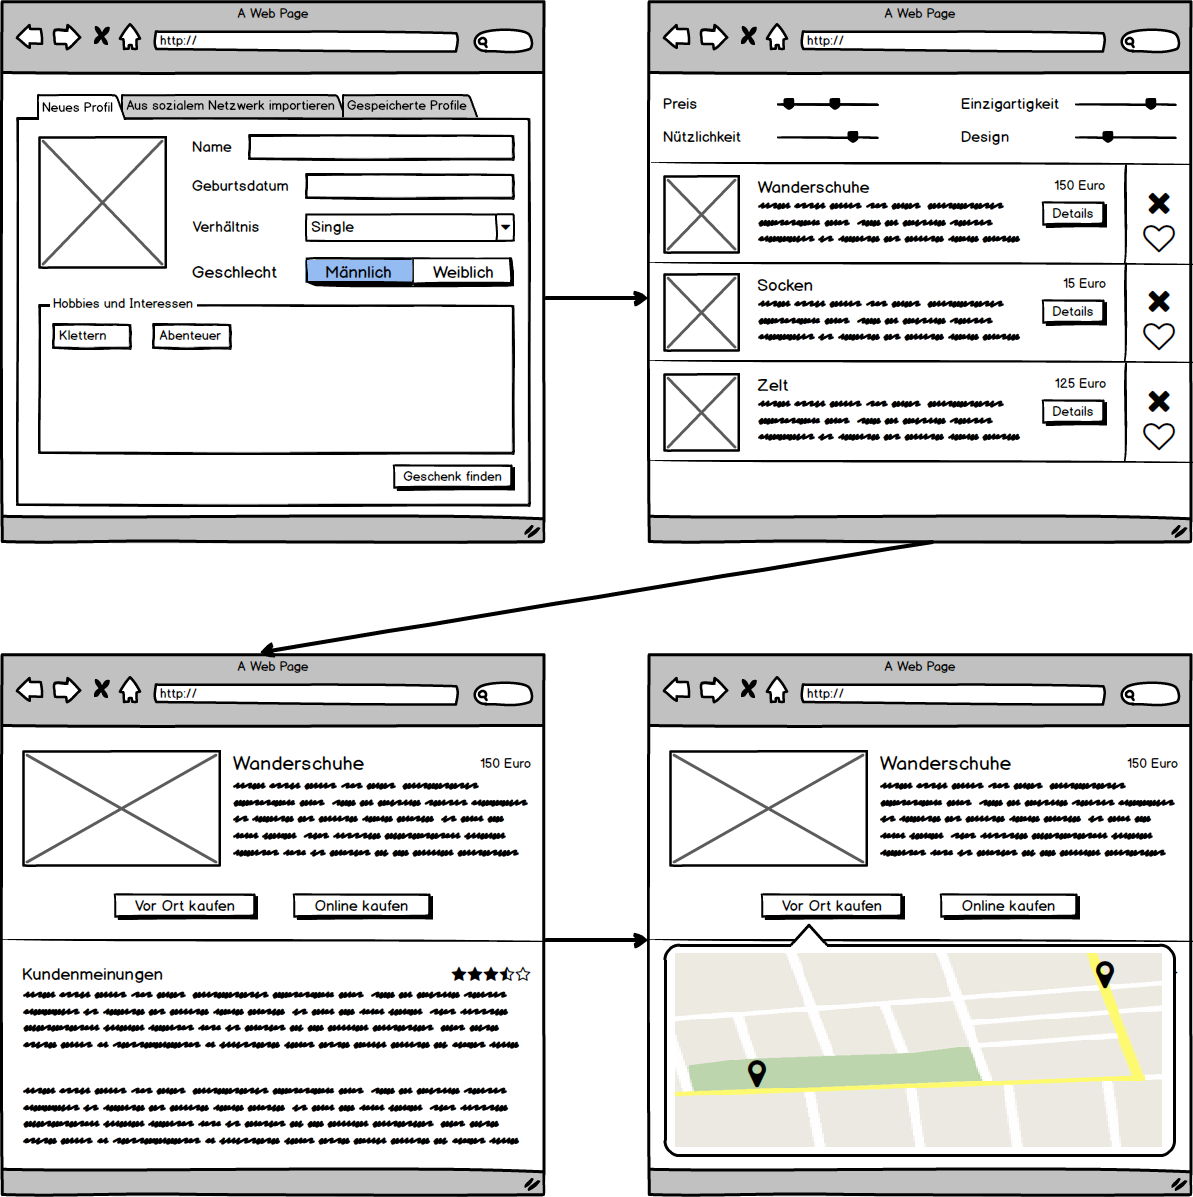
\includegraphics[width=0.83\paperwidth,height=0.65\paperheight]{prt3}}
    \caption{Webseite (Prototyp 3)}
    \label{fig:prt3}
\end{figure}

\begin{figure}[ht]
    \centering
      \makebox[\textwidth]{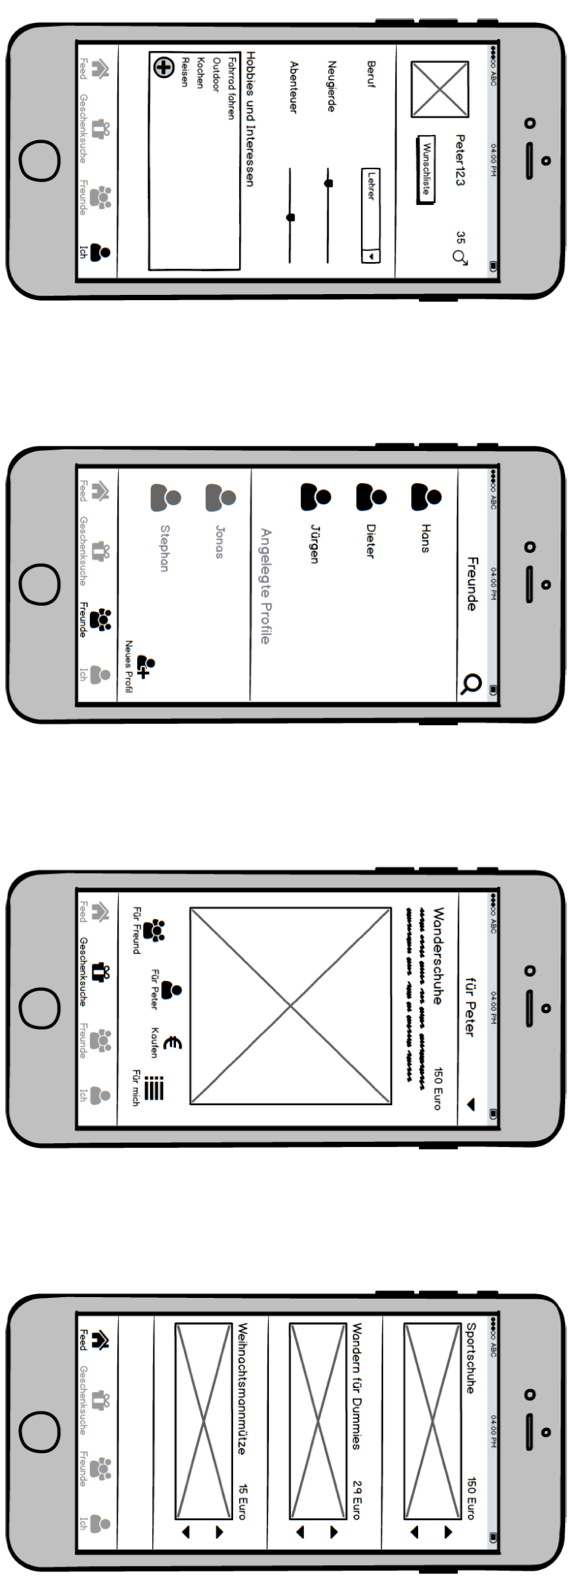
\includegraphics[height=0.8\paperheight]{prt4}}
    \caption{Soziales Netz (Prototyp 4)}
    \label{fig:prt4}
\end{figure}
